\section{Desarrollo.}
El Sistema Informático desarrollado se compone de 3 módulos / elementos que de forma conjunta proveen de la funcionalidad necesaria a AutoCAD para exportar los elementos del fichero DWG a un fichero en un formato XML. Estos módulos se apoyan en los siguientes componentes que el propio AutoCAD expone a disposición de los desarrolladores:

\begin{itemize}

\item{AutoDesk.AutoCAD.Runtime: este módulo inicializa los servicios de la aplicación cliente y las factorias que producen los diferentes objetos para ser utilizados dentro del entorno .NET.}

\item{AutoDesk.AutoCAD.ApplicationServices: este módulo permite la interacción con la aplicación AutoCAD. Provee acceso a los módulos adicionales como el editor, el gestor de documentos, ventana principal, etc.}

\item{AutoDesk.AutoCAD.DatabaseServices: esto módulo permite la interacción con el fichero de dibujo AutoCAD (DWG). Permite el acceso al header del mismo, a las tablas de símbolos, a las tablas de registros de entidades y a los diferentes objetos que componen el dibujo.}

\item{AutoDesk.AutoCAD.Geometry: esto modulo permite la interacción con el servicio de geometría de AutoCAD que se encarga de la gestión de las referencias espaciales.}

\item{AutoDesk.AutoCAD.EditorInput: esto modulo permite la interacción con el editor a través del cual se realiza la interacción con el usuario en ambos sentidos.}

\end{itemize}

Los 3 módulos / elementos desarrollados son:

\begin{itemize}

\item{dwgElementos: este módulo contiene las clases necesarias para representar y almacenar en memoria la información contenida en un fichero con formato DWG. En concreto esta formado por las clases:}

\begin{itemize}

\item{dwgPunto: representa un punto de un plano de AutoCAD.}
\item{dwgLinea: representa una línea de un plano de AutoCAD.}
\item{dwgArco: representa un arco de un plano de AutoCAD. También contiene la representación equivalente del arco como un conjunto de líneas.}
\item{dwgPolylinea: representa una polilinea de un plano de AutoCAd. También contiene la representación equivalente de la polilinea como un conjunto de líneas y arcos.}
\item{dwgCapa: representa una capa de un plano de AutoCAD.}
\item{dwgFile: representa un fichero DWG conteniendo toda la informaciónd del mismo relativa a capas, puntos, líneas, polilineas y arcos.}

\end{itemize}

A continuación se muestra un diagrama UML de este módulo dwgElementos:

\begin{figure}[H]
\begin{center}
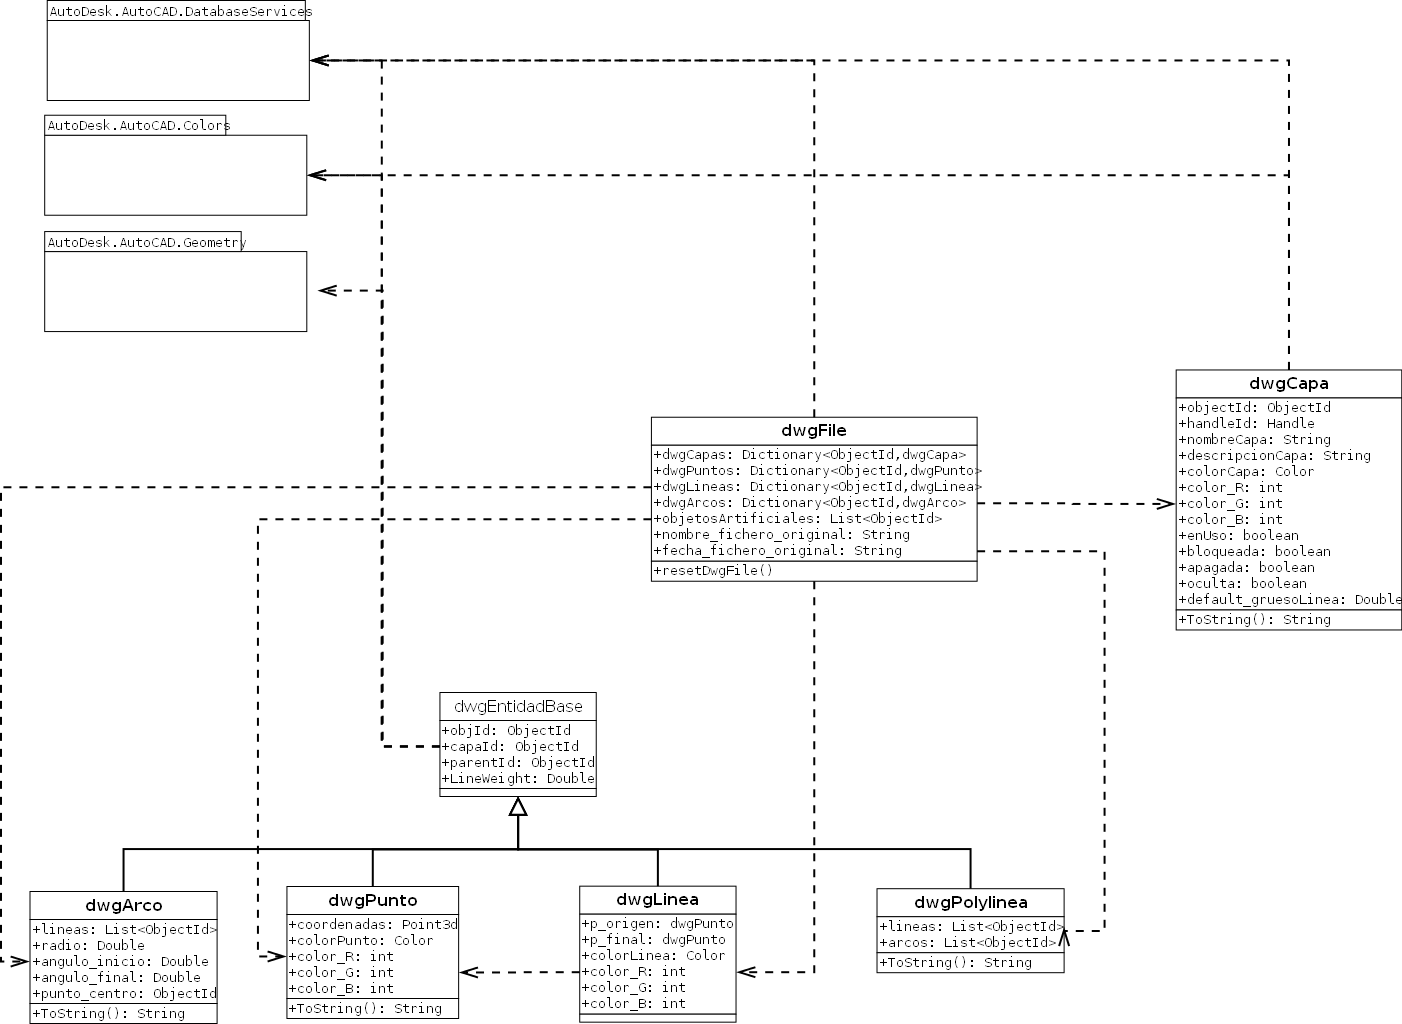
\includegraphics[width=0.65\textwidth]{imgs/dwgElementos}
\caption{Diagrama UML del módulo dwgElementos.}
\end{center}
\end{figure}

\item{dwgTools: este módulo contiene las clases de apoyo y herramientas necesarias para completar el proceso de extracción de la información del fichero DWG. En concreto, esta formado por las clases:}

\begin{itemize}

\item{herramientasCurvas: contiene las clases y métodos necesarios para transformar una curva en un conjunto de líneas rectas equivalentes.}
\item{exportXMl: contiene las clases y métodos necesarios para exportar el contenido representado en memoria a través del módulo dwgElementos a un fichero de texto.}

\end{itemize}

\item{dwgDecoder: módulo principal que implementa el plugin de AutoCAD apoyándose en los dos módulos anteriores. A continuación se muestra un diagrama UML que realaciona todos los elementos:}

\begin{figure}[H]
\begin{center}
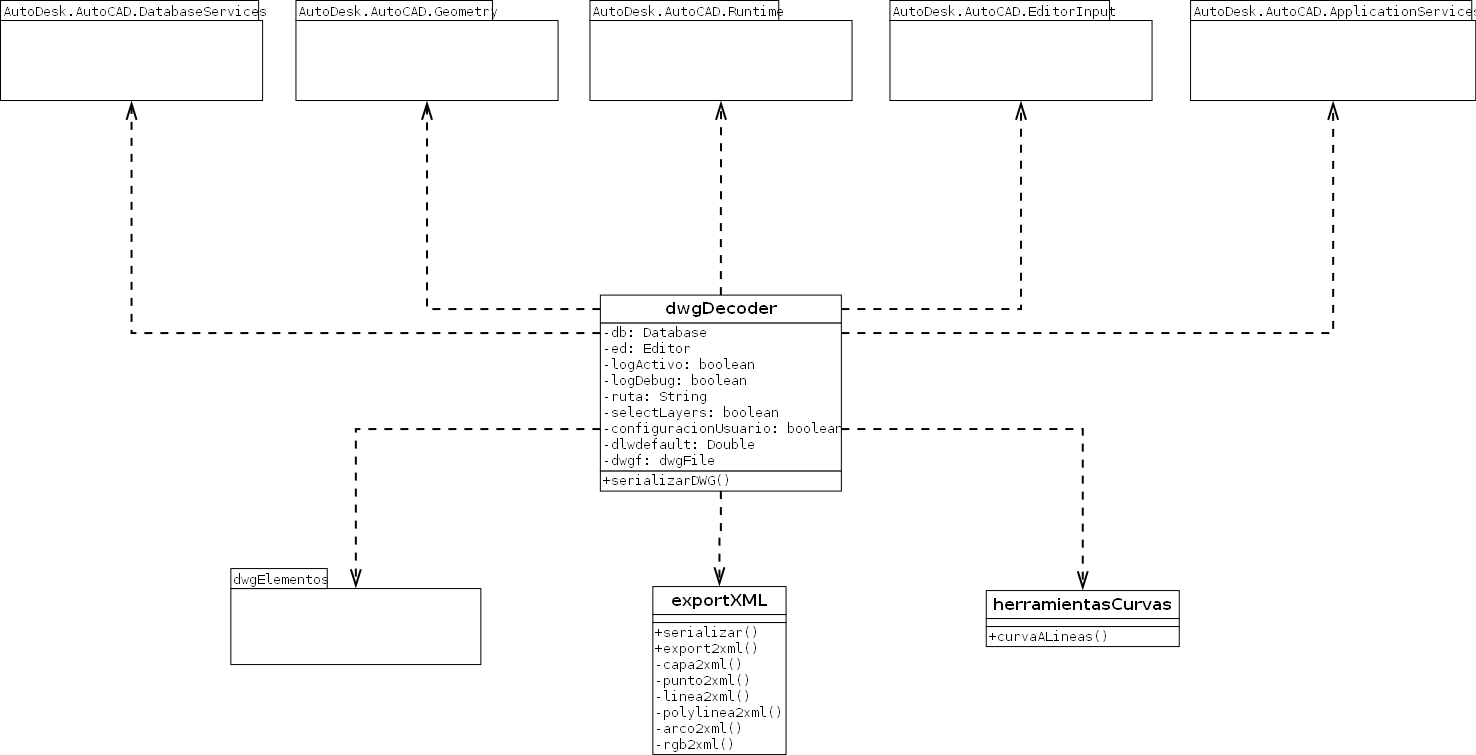
\includegraphics[width=0.65\textwidth]{imgs/dwgDecoder}
\caption{Diagrama UML del sistema dwgDecoder.}
\end{center}
\end{figure}

El proceso de decodificación se compone de 4 etapas. La primera de ellas corresponde con la configuración del proceso donde se solicita al usuario si desea un log del proceso y el grado de detalle de la información del mismo, la ruta donde se almacenará el fichero de salida y si desea seleccionar manualmente las capas a incluir en el proceso de extracción. A continuación se muestra el diagrama de flujo correspondiente a esta etapa:

\begin{figure}[H]
\begin{center}
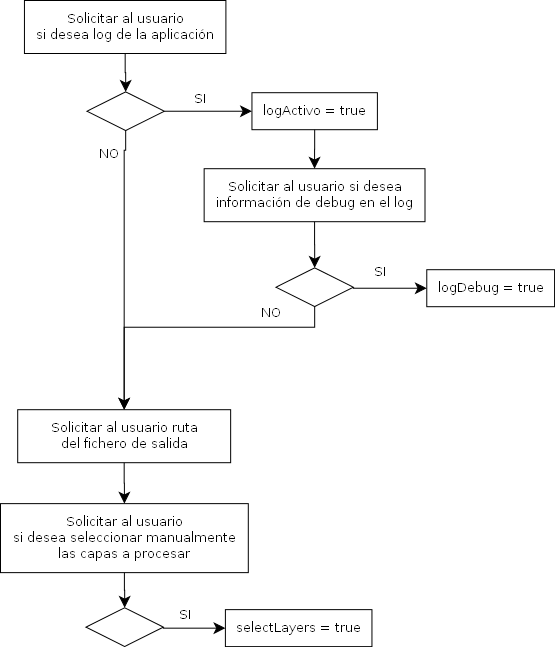
\includegraphics[width=0.65\textwidth]{imgs/diagramaFlujo}
\caption{Diagrama de flujo de la etapa de configuración.}
\end{center}
\end{figure}

En una segunda etapa se examinan todas las capas existentes en el fichero y si el usuario ha indicado que quiere seleccionar manualmente las capas a procesar se le va preguntando por cada una ellas para que decida si su información debe ser interpretada. Si el usuario no ha indicado que quiere hacer una selección manual se obtiene e interpreta la información de todas las capas. A continuación se muestra el digrama de flujo correspondiente a esta etapa:

\begin{figure}[H]
\begin{center}
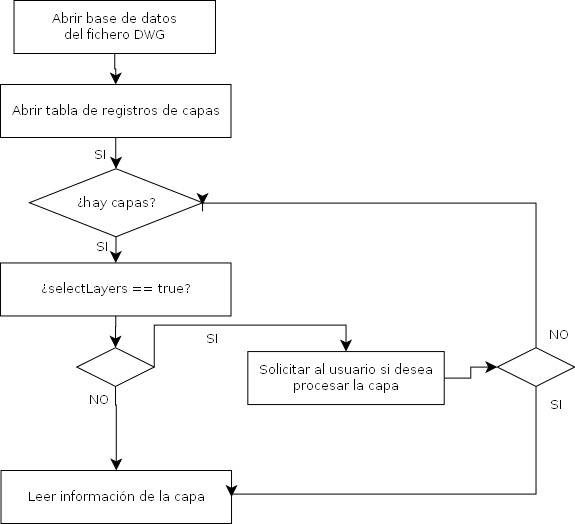
\includegraphics[width=0.65\textwidth]{imgs/diagramaFlujo2}
\caption{Diagrama de flujo de la etapa de lectura de capas.}
\end{center}
\end{figure}

En una tercera etapa se examinan todos objetos existentes dentro del fichero DWG. Si el objeto esta en una de las capas que debe ser procesada, se interpreta la información del objeto y se incorpora al contenido del objeto de tipo dwgFile. En el caso de los objetos polilínea y arco se descomponen en líneas simples antes de ser incorporados al objeto de tipo dwgFile. A continuación se muestra el digrama de flujo correspondiente a esta etapa:

\begin{figure}[H]
\begin{center}
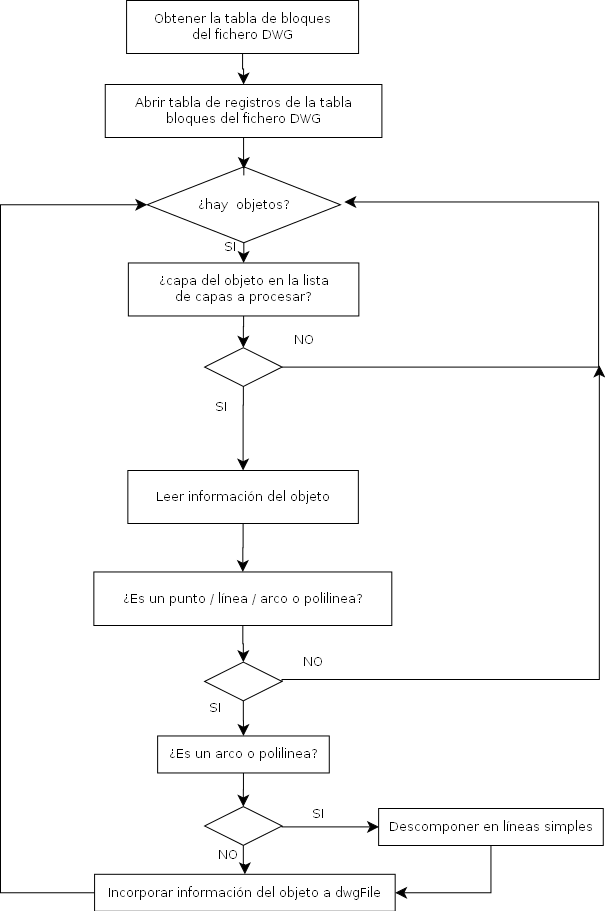
\includegraphics[width=0.65\textwidth]{imgs/diagramaFlujo3}
\caption{Diagrama de flujo de la etapa de lectura de objetos.}
\end{center}
\end{figure}

En una cuarta y última etapa se vuelca todo el contenido del objeto dwgFile a un fichero de texto en formato XML almacenándolo en la ruta indicada por el usuario durante el proceso de configuración del proceso de extracción.

\end{itemize}
